\chapter{Fundamentação teórica}\label{cap:revisao}

Nesta seção será discutido o funcionamento e as principais características do LZ77 e do algoritmo aritmético, com o propósito de permitir ao leitor uma melhor compreensão dos algoritmos utilizados neste trabalho.

\section{Funcionamento do LZ77}\label{sec:LZ77}

O algoritmo de compressão LZ77, proposto por Ziv e Lempel em 1977~\cite{1055714}, pertence à classe dos métodos baseados em dicionário. No LZ77, o dicionário é construído dinamicamente a partir de partes já codificadas da própria entrada, o que dispensa a necessidade de um dicionário fixo ou pré-definido. Este é utilizado como base em algoritmos amplamente adotados, como o DEFLATE.

Para realizar a codificação, o algoritmo utiliza uma janela deslizante que percorre a sequência de entrada. Essa janela é dividida em duas regiões principais:

\begin{itemize}
  \item \textbf{\textit{Search buffer}}: contém a porção já codificada da sequência, armazenando até $n$~caracteres recentes. Ele funciona como o “dicionário” atual, onde o codificador tenta encontrar correspondências com os próximos caracteres a serem codificados.
  \item \textbf{\textit{Lookahead buffer}}: armazena os próximos caracteres a serem analisados e codificados. O codificador busca no \textit{search buffer} a maior sequência que coincida com os caracteres do \textit{lookahead buffer}.
\end{itemize}

Durante a codificação, o algoritmo utiliza um ponteiro de correspondência (\textit{match pointer}) que percorre o \textit{search buffer} para identificar o maior prefixo do \textit{lookahead buffer} que também ocorra ali. Quando uma correspondência é encontrada, ela é codificada como um trio $\langle o, l, c \rangle$, onde:
\begin{itemize}
  \item $o$ (\textit{offset}): distância entre o início da correspondência no \textit{search buffer} e a posição atual da janela;
  \item $l$ (\textit{length}): comprimento da sequência que será codificada;
  \item $c$ (\textit{character}): próximo caractere literal após a sequência correspondente.
\end{itemize}

A Figura~\ref{fig:Diagrama LZ77} ilustra essa estrutura, destacando as divisões da janela deslizante e o funcionamento da busca por correspondências.

\begin{figure}[ht]
	\centering
	\caption{Divisão da janela deslizante no algoritmo LZ77}
	\label{fig:Diagrama LZ77}
	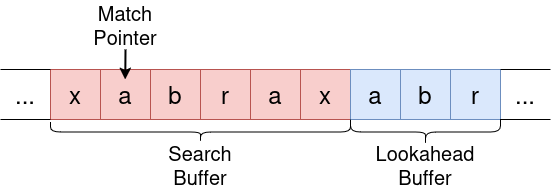
\includegraphics[width=12cm]{figuras/DiagramasTCC-LZ77-template}
    \fonte{Adaptada de \textcite{sayood2012introduction}}
\end{figure}

Este mecanismo permite substituir sequências repetidas por referências a ocorrências anteriores, resultando em compressões eficazes especialmente para dados com alta redundância.

\subsection{Exemplo de Codificação com LZ77}\label{sec:LZ77_exemplo}

Nesta seção será demonstrado um exemplo detalhado do funcionamento da janela deslizante e da representação do trio $\langle o, l, c \rangle$ utilizados pelo algoritmo LZ77. A sequência a ser codificada é \texttt{"cabracadabrarrarrad"}. Para este exemplo, a janela deslizante possui um tamanho total fixo de 13 caracteres, com o \textit{lookahead buffer} definido em 6 caracteres. O estado inicial da janela pode ser visto na Figura~\ref{fig:Estado_0_LZ77}.

\begin{figure}[ht]
\centering
\caption{Estado inicial da janela deslizante no algoritmo LZ77}
\label{fig:Estado_0_LZ77}
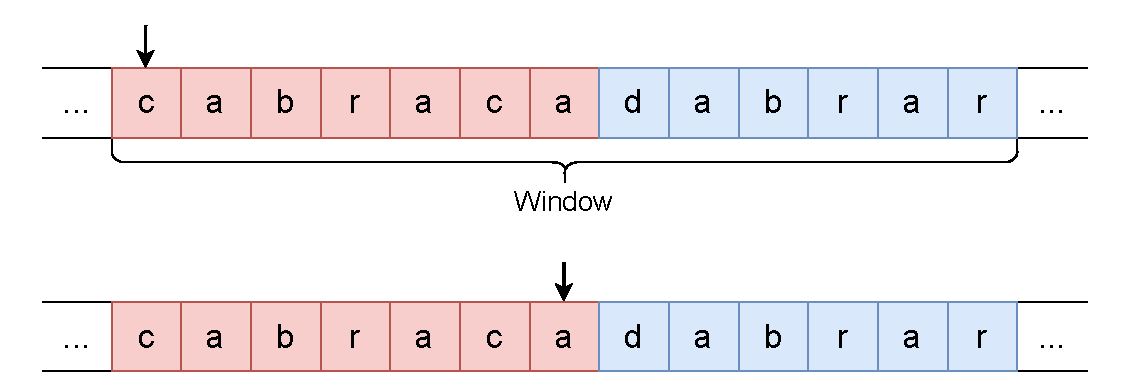
\includegraphics[width=15cm]{figuras/DiagramasTCC-LZ77-Estado-0}
\fonte{Adaptada de \textcite{sayood2012introduction}}
\end{figure}

Inicialmente, busca-se no \textit{search buffer} algum caractere ou sequência que coincida com o início do \textit{lookahead buffer}. Neste momento, deseja-se codificar o primeiro caractere do \textit{lookahead buffer}, que é \texttt{"d"}. Ao observar o \textit{search buffer}, verifica-se que não há nenhuma correspondência prévia para este caractere. Portanto, o algoritmo gera o trio $\langle 0, 0, \texttt{d} \rangle$, indicando que não houve correspondência ($0$ de deslocamento e $0$ de comprimento) e que o caractere literal transmitido é \texttt{"d"}.

Após esta codificação inicial, a janela deslizante avança uma posição, o que altera o conteúdo tanto do \textit{search buffer} quanto do \textit{lookahead buffer}, conforme mostrado na Figura~\ref{fig:Estado_1_LZ77}.

\begin{figure}[ht]
\centering
\caption{Estado da janela após primeira codificação no algoritmo LZ77}
\label{fig:Estado_1_LZ77}
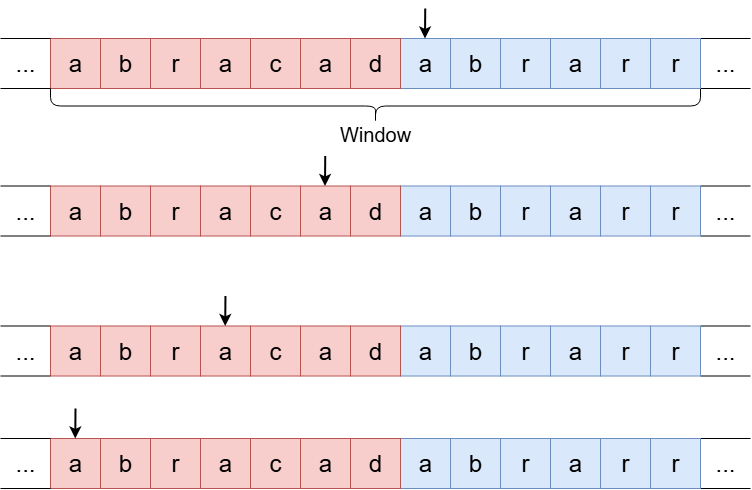
\includegraphics[width=15cm]{figuras/DiagramasTCC-LZ77-Estado-1}
\fonte{Adaptada de \textcite{sayood2012introduction}}
\end{figure}

Nesse novo estado, procura-se novamente uma correspondência no \textit{search buffer} para a sequência do \textit{lookahead buffer}, que agora começa com \texttt{"a"}. Observando o \textit{search buffer}, é possível encontrar múltiplas ocorrências isoladas do caractere \texttt{"a"}, porém, busca-se sempre a correspondência mais longa possível. Notavelmente, existe uma sequência completa \texttt{"abra"} previamente codificada, iniciando a 7~caracteres de distância da posição atual da janela. Essa correspondência possui comprimento 4~caracteres.

Dessa forma, o algoritmo codifica a sequência encontrada como o trio $\langle 7, 4, \texttt{r} \rangle$, onde $7$ indica a distância até o início da correspondência no \textit{search buffer}, $4$ indica o comprimento da correspondência encontrada (\texttt{"abra"}), e \texttt{"r"} é o caractere seguinte imediatamente após essa sequência, ainda não codificado. Após isso, a janela avança em 5~posições (4~caracteres da sequência codificada mais 1~caractere literal).

Para realizar o processo inverso, ou seja, decodificar o trio recebido $\langle 7, 4, \texttt{r} \rangle$, o decodificador utiliza o mesmo princípio do algoritmo LZ77, porém no sentido inverso.

Inicialmente, ele utiliza o offset ($o$) para retornar exatamente 7 posições na sequência já decodificada até o momento. A partir dessa posição inicial encontrada, copia-se uma sequência de comprimento 4 (valor $l$), obtendo o trecho \texttt{"abra"}. Em seguida, adiciona-se ao final desta sequência copiada o caractere literal adicional ($c$), que neste exemplo é \texttt{"r"}.

Esse processo é ilustrado passo a passo na Figura~\ref{fig:Estado_deconding}. Inicialmente, há o estado parcial da decodificação com o \textit{buffer} já reconstruído. Em seguida, avança-se caractere a caractere, copiando-se do \textit{buffer} reconstruído e adicionando o caractere literal no final. O resultado final após a decodificação deste trio será \texttt{"abrar"}.

Vale destacar que o decodificador reconstrói o buffer de busca dinamicamente, conforme recebe e processa novos trios, permitindo a reconstrução exata dos dados originais sem perda alguma.

% Até Aqui

\begin{figure}[ht]
\centering
\caption{Decodificação do exemplo $\langle 7, 4, \texttt{r} \rangle$ }
\label{fig:Estado_deconding}
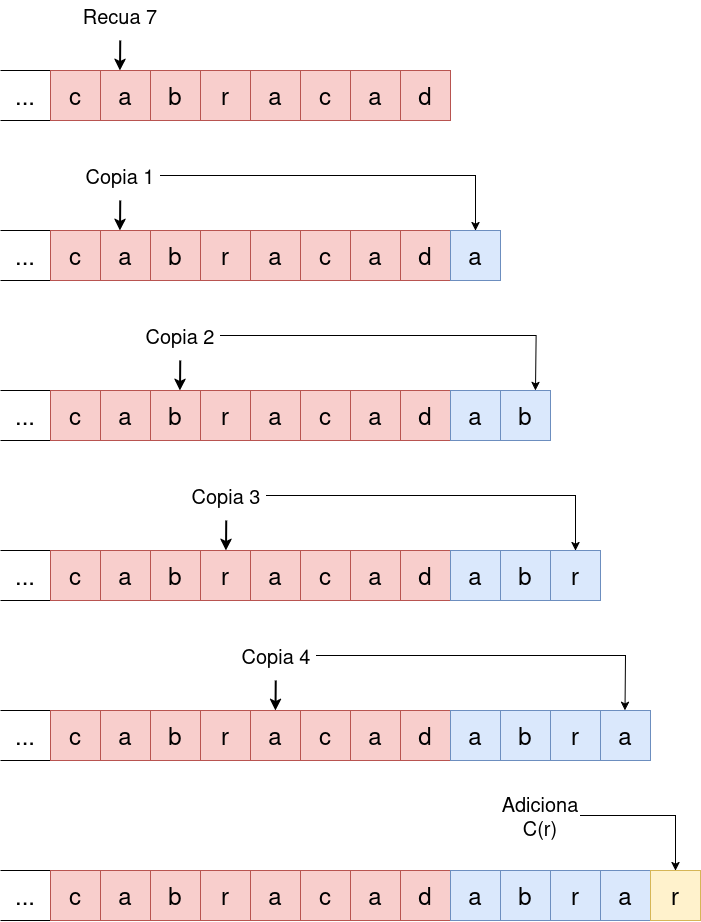
\includegraphics[width=12cm]{figuras/DiagramasTCC-LZ77-Decoding}
\fonte{Adaptada de \textcite{sayood2012introduction}}
\end{figure}

Utilizando o exemplo anterior do trio $\langle 7, 4, \texttt{r} \rangle$, onde a janela total possui 13 caracteres, temos a seguinte definição dos campos em bits:
\begin{itemize}
  \item O deslocamento ($o$) pode variar de 0 a 7, portanto requer $3$~bits;
  \item  O comprimento ($l$) pode variar de 0 a 6, logo exige também $3$~bits;
  \item O caractere literal ($c$) é codificado em ASCII, utilizando $8$~bits ($1$~byte).
\end{itemize}
Dado que na implementação adotada os tamanhos em bits para cada campo do trio são
\[
\underbrace{3}_{\substack{\text{bits para}\\\text{offset }(o)}} + 
\underbrace{3}_{\substack{\text{bits para}\\\text{length }(l)}} + 
\underbrace{8}_{\substack{\text{bits para}\\\text{character }(c)}} 
= 14\;\text{bits},
\]
temos um formato de código de comprimento fixo, no qual cada trio $\langle o, l, c\rangle$ ocupará exatamente 14 bits. Em outras palavras, após definido o tamanho da janela (\textit{offset}) e do \textit{lookahead buffer} (\textit{length}), bem como o padrão de 8 bits para o caractere literal, toda e qualquer codificação produzida por esse esquema terá comprimento contínuo de 14 bits por símbolo codificado \cite{nelson2008data}.

Realizando a codificação especificamente para o exemplo dado ($\langle 7, 4, \texttt{r} \rangle$), obtêm-se:
\begin{itemize}
  \item O valor do \textit{offset} $o = 7$, em $3$ bits é $111_{(2)}$.
  \item O comprimento $l = 4$, em $3$ bits é $100_{(2)}$.
  \item O caractere $r$, em ASCII binário ($8$ bits), é $01110010_{(2)}$.
\end{itemize}
Portanto, a representação completa do trio em bits será:
$$
111 \;|\; 100 \;|\; 01110010
$$
Resultando na sequência binária final: $11110001110010_{(2)}$.

Esse processo ilustra o funcionamento fundamental do algoritmo LZ77, mostrando como ele explora redundâncias por meio de correspondências encontradas em trechos já codificados, reduzindo o volume de dados transmitidos ou armazenados.

% Revisões Aqui
\section{Algoritmo aritmético}\label{Algoritmo aritmético}

O algoritmo aritmético de compressão foi desenvolvido simultaneamente por Jorma J. Rissanen, da IBM Research, e por Richard Pasco, da Universidade de Stanford, tendo ambos publicado seus artigos em maio de 1976~\cite{10.5555/908099},~\cite{5391119}. Para uma explicação mais detalhada, pode-se consultar também a série de vídeos \texttt{"Information Theory"} por mathematicalmonk

O algoritmo aritmético é um método de codificação por fluxo (\textit{stream code}) que representa uma sequência completa de símbolos por meio de um único número real fracionário pertencente ao intervalo $[0,1[$. Considerando que o conjunto dos números reais nesse intervalo é infinito, torna-se possível atribuir uma \textit{tag} exclusiva para cada sequência distinta de símbolos, estreitando progressivamente esse intervalo conforme cada símbolo é processado.

Ao contrário de métodos que atribuem códigos fixos ou códigos prefixos, como o Huffman, o algoritmo aritmético utiliza diretamente as probabilidades de cada símbolo para subdividir e refinar o intervalo, alcançando, teoricamente, taxas de compressão próximas ao limite da entropia da fonte.

\subsection{Algoritmo com precisão infinita}

Para esta primeira análise, será assumido que não há problemas relacionados à divisão infinita dos valores. Portanto, supõe-se precisão infinita durante os cálculos realizados pelo algoritmo.

\textbf{Observação:} Na codificação aritmética é comum, e altamente recomendável, reservar um símbolo especial para indicar o fim da mensagem, conhecido como \textit{End of File} (EoF). Isso se deve ao fato de que a codificação resulta em um único número fracionário e, sem o EoF, o decodificador não teria como saber quando a mensagem termina, a menos que o seu comprimento total seja previamente conhecido. O uso de um símbolo EoF torna a decodificação autossuficiente e precisa.


Considere o exemplo definido pelos seguintes parâmetros:
\[
\begin{aligned}
X &= \{a, b, c\} \\
\text{EoF (End of File)} &:\; a \\
p &= (p_1, p_2, p_3) = (p_a, p_b, p_c) \\
p &= (p_1, p_2, p_3) = (0.2,\, 0.4,\, 0.4) \\
c &= (c_1, c_2, c_3) = (0,\, 0.2,\, 0.6)
\end{aligned}
\]
onde:
\begin{itemize}
  \item $X$ é o alfabeto dos símbolos possíveis;
  \item $\text{EoF}$ (End of File) é o símbolo especial que indica o fim da sequência;
  \item $p_i$ é a probabilidade individual associada a cada símbolo $i$;
  \item $c_i$ é a probabilidade acumulada, definida por:
\[
c_i = \sum_{j=0}^{i-1} p_j.
\]
\end{itemize}

A Figura~\ref{fig:Diagramas-Aritmetic-Encoding} ilustra o processo de codificação aritmética para a sequência \texttt{"cba"}.

\begin{figure}[ht]
	\centering
	\caption{Codificação da palavra \texttt{"cba"} utilizando codificação aritmética}
	\label{fig:Diagramas-Aritmetic-Encoding}
	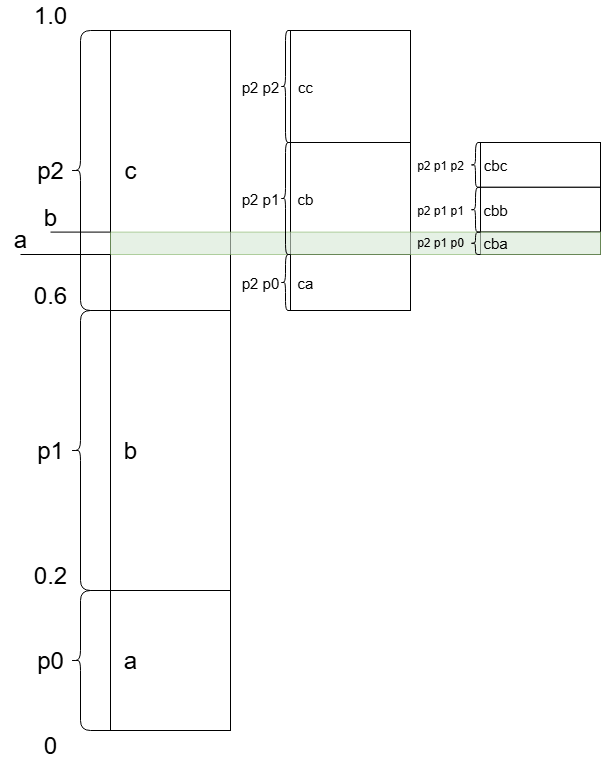
\includegraphics[width=13cm]{figuras/DiagramasTCC-Aritmetic-Encoding}
    \fonte{Elaborada pelo autor}
\end{figure}

O fluxo de codificação é contínuo, e todos os símbolos da mensagem são codificados de forma conjunta. Isso resulta em um código dinâmico, particularmente eficiente para fontes com distribuições probabilísticas variáveis.

O processo inicia com o intervalo inicial $[low, high[ = [0, 1[$. A cada símbolo processado, esse intervalo é subdividido proporcionalmente às probabilidades acumuladas dos símbolos.

Formalmente, para cada símbolo $s$ correspondente ao índice $j$, o subintervalo é calculado por
\[
[\,low + (high - low) c_{j-1},\; low + (high - low) c_j\,[\,,
\]
garantindo que a largura do subintervalo resultante seja exatamente a probabilidade associada ao símbolo.

Aplicando esses cálculos ao exemplo, os subintervalos a cada etapa ficam definidos da seguinte maneira:

\begin{enumerate}
    \item \textbf{Símbolo \texttt{"c"}}:
    \[
    [\,low, high\,[ ~~ = ~ [\,c_2,\; c_2 + p_2\,[ ~~ = ~ [\,0{,}6;\;1\,[\,.
    \]

    \item \textbf{Símbolo \texttt{"b"}} (novo intervalo sobre o intervalo anterior):
    \[
    [\,low, high\,[ = [\,0{,}6 + (1 - 0{,}6)\cdot c_1,\; 0{,}6 + (1 - 0{,}6)\cdot (c_1 + p_1)\,[ = [\,0{,}68;\;0{,}84\,[\,.
    \]

    \item \textbf{Símbolo \texttt{"a"}} (novo intervalo sobre o intervalo anterior):
    \[
    [\,low, high\,[ = [\,0{,}68 + (0{,}84 - 0{,}68)\cdot c_0,\; 0{,}68 + (0{,}84 - 0{,}68)\cdot (c_0 + p_0)\,[ = [\,0{,}68;\;0{,}712\,[\,.
    \]
\end{enumerate}

Esse intervalo final representa a sequência completa codificada.

\begin{figure}[ht]
	\centering
	\caption{Codificação da palavra \texttt{"cba"} em bits}
	\label{fig:DiagramasTCC-Diagramas-Aritmetic-Encoding-Bits}
	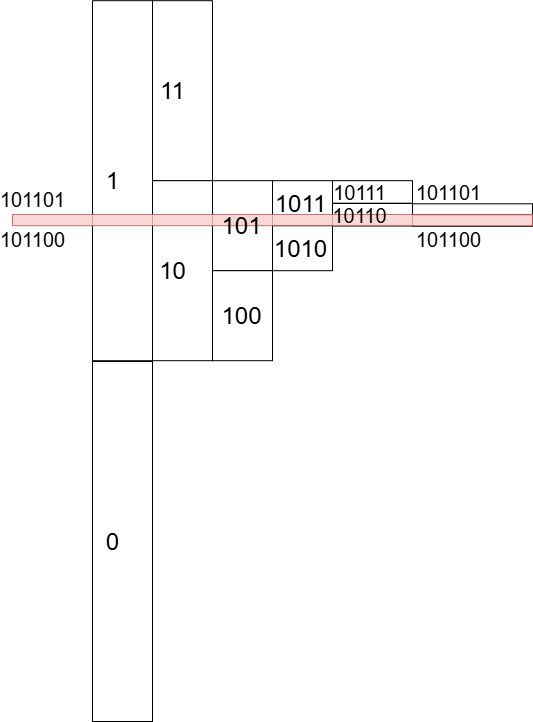
\includegraphics[width=10cm]{figuras/DiagramasTCC-Diagramas-Aritmetic-Encoding-Bits}
    \fonte{Elaborada pelo autor}
\end{figure}


No exemplo em questão, o intervalo final de codificação é \([0{,}68;0{,}712[\). A árvore de subdivisões mostra:
\begin{itemize}
  \item A primeira divisão \(\{0,1\}\) separa \([0; 0{,}5[\) e \([0{,}5; 1[\). Como o nosso intervalo está em \([0{,}68; 0{,}712[\), ele pertence à segunda metade, logo o primeiro bit é \texttt{"1"}.
  \item Em seguida, subdivide-se \([0{,}5,1[\) em \([0{,}5; 0{,}75[\) (prefixo \texttt{"10"}) e \([0{,}75{;}1[\) (prefixo \texttt{"11"}). Visto que ainda estamos em \([0{,}68; 0{,}712[\subset[0{,}5; 0{,}75[\), o segundo bit é \texttt{"0"}, formando o prefixo \texttt{"10"}.
  \item O processo continua, refinando o intervalo \texttt{"10"} em \texttt{"100"} vs.\ \texttt{"101"} e assim por diante, até que o prefixo binário completo caia estritamente dentro de \([0{,}68;0{,}712[\). 
\end{itemize}

Observando o diagrama, chegamos ao prefixo
\[
\mathtt{0.101100_2}
\]
que define o subintervalo $[\mathtt{0.101100_2}, \mathtt{0.101101_2}[ ~~ = ~ [0{,}6875;0{,}703125[$, inteiramente contido em $[0{,}68;0{,}712[$. Assim, a sequência \texttt{"101100"} é a codificação em bits de precisão mínima que captura fielmente o valor fracionário representativo da mensagem original usando precisão efetivamente infinita.

%Até aquiequência completa codificada.

Para converter o intervalo final em uma sequência de bits, considera-se inicialmente a representação infinita do espaço \([0,1[\) em subdivisões binárias. Cada dígito binário (\texttt{"0"} ou \texttt{"1"}) corresponde a uma metade do intervalo atual, conforme ilustra o diagrama da Figura~\ref{fig:DiagramasTCC-Diagramas-Aritmetic-Encoding-Bits}. A codificação prossegue extraindo o menor prefixo binário que, como número real, cai totalmente dentro do intervalo final calculado para a sequência \texttt{"cba"}. 

\subsection{Algoritmo com Precisão Finita e Redimensionamento}

A análise realizada anteriormente considera que o algoritmo aritmético dispõe de precisão infinita nos cálculos numéricos. Porém, em implementações práticas, é necessário adaptar o algoritmo para trabalhar com precisão finita, já que computadores apresentam limitações na precisão dos números de ponto flutuante.

Essa adaptação consiste na aplicação periódica de uma operação chamada de \textit{redimensionamento} (\textit{rescaling}), cujo objetivo é evitar que o intervalo codificado torne-se pequeno demais, causando perda numérica de precisão. O procedimento de redimensionamento é ilustrado na Figura~\ref{fig:DiagramasTCC-Aritmetic-Rescaling}.

\begin{figure}[ht]
	\centering
	\caption{Operação geral de redimensionamento na codificação aritmética}
	\label{fig:DiagramasTCC-Aritmetic-Rescaling}
	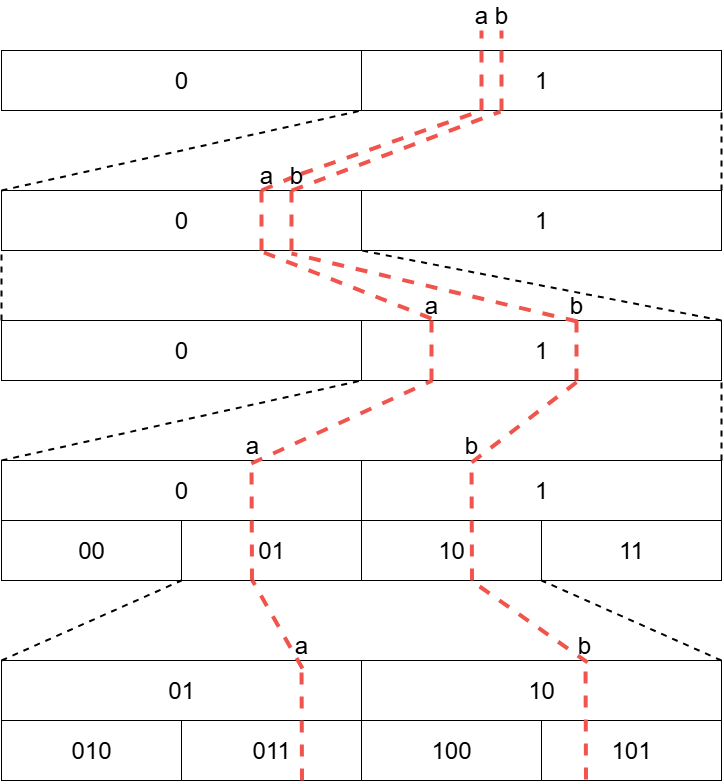
\includegraphics[width=13cm]{figuras/DiagramasTCC-Aritmetic-Rescaling}
    \fonte{Elaborada pelo autor}
\end{figure}


Esse procedimento pode ser descrito pelos seguintes critérios básicos:

\begin{enumerate}
    \item \textbf{Caso \( b < \frac{1}{2} \):} 
    Quando todo o intervalo atual estiver na primeira metade do intervalo [0,1[, ou seja, \( [a,b[ \subset [0,\frac{1}{2}[ \), emite-se o bit `0' e realiza-se o escalonamento:
    \[
    a \leftarrow 2 \cdot a, \quad b \leftarrow 2 \cdot b
    \]
    conforme Figura~\ref{fig:DiagramasTCC-Diagramas-Aritmetic-Rescaling-0}.

    \item \textbf{Caso \( a \geq \frac{1}{2} \):}
    Quando todo o intervalo atual estiver na segunda metade do intervalo, \( [a,b[ \subset [\frac{1}{2},1[ \), emite-se o bit `1' e efetua-se o redimensionamento do intervalo:
    \[
    a \leftarrow 2 \cdot \left(a - \frac{1}{2}\right), \quad b \leftarrow 2 \cdot \left(b - \frac{1}{2}\right)
    \]
    ilustrado na Figura~\ref{fig:DiagramasTCC-Diagramas-Aritmetic-Rescaling-1}.

    \item \textbf{Caso \( a \geq \frac{1}{4} \) e \( b < \frac{3}{4} \):}
    Quando o intervalo codificado situa-se na metade central do intervalo unitário, ou seja, entre \( \frac{1}{4} \) e \( \frac{3}{4} \), é necessário utilizar um contador \( s \), inicialmente igual a zero, que indica a quantidade de redimensionamentos consecutivos ocorridos nesse caso intermediário. Aplica-se o escalonamento:
    \[
    a \leftarrow 2 \cdot \left(a - \frac{1}{4}\right), \quad b \leftarrow 2 \cdot \left(b - \frac{1}{4}\right), \quad s \leftarrow s + 1
    \]
    Essa operação é ilustrada na Figura~\ref{fig:DiagramasTCC-Diagramas-Aritmetic-Rescaling-S}. O contador \( s \) registra a quantidade de bits ainda pendentes a serem emitidos.

    Quando finalmente o intervalo migrar para uma das metades externas do intervalo, será emitido o bit correspondente (`0' ou `1'), seguido por \( s \) bits adicionais complementares (se o bit emitido for `0', os \( s \) bits seguintes serão `1', e vice-versa). Após a emissão, o contador \( s \) é zerado.

\end{enumerate}

As Figuras~\ref{fig:DiagramasTCC-Diagramas-Aritmetic-Rescaling-0}, \ref{fig:DiagramasTCC-Diagramas-Aritmetic-Rescaling-1} e \ref{fig:DiagramasTCC-Diagramas-Aritmetic-Rescaling-S} exemplificam detalhadamente esses critérios.

\begin{figure}[ht]
	\centering
	\caption{Redimensionamento quando \( b < \frac{1}{2} \)}
	\label{fig:DiagramasTCC-Diagramas-Aritmetic-Rescaling-0}
	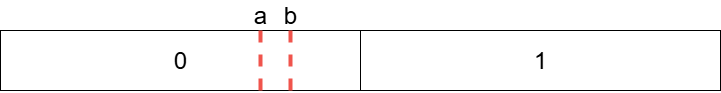
\includegraphics[width=12cm]{figuras/DiagramasTCC-Diagramas-Aritmetic-Rescaling-0}
    \fonte{Elaborada pelo autor}
\end{figure}

\begin{figure}[ht]
	\centering
	\caption{Redimensionamento quando \( a \geq \frac{1}{2} \)}
	\label{fig:DiagramasTCC-Diagramas-Aritmetic-Rescaling-1}
	
\includegraphics[width=12cm]{figuras/DiagramasTCC-Diagramas-Aritmetic-Rescaling-1}
    \fonte{Elaborada pelo autor}
\end{figure}

\begin{figure}[ht]
	\centering
	\caption{Redimensionamento quando o intervalo está na metade central \( \frac{1}{4} \leq a < b < \frac{3}{4} \)}
	\label{fig:DiagramasTCC-Diagramas-Aritmetic-Rescaling-S}
	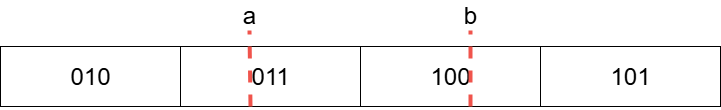
\includegraphics[width=12cm]{figuras/DiagramasTCC-Diagramas-Aritmetic-Rescaling-S}
    \fonte{Elaborada pelo autor}
\end{figure}

Além desses critérios básicos, também podem ocorrer subdivisões adicionais específicas, mostradas nas Figuras~\ref{fig:DiagramasTCC-Diagramas-Aritmetic-Rescaling-3Q} e \ref{fig:DiagramasTCC-Diagramas-Aritmetic-Rescaling-Q}, onde são detalhadas subdivisões específicas adicionais.

\begin{figure}[ht]
	\centering
	\caption{Subdivisão específica em \( \frac{3}{4} \)}
	\label{fig:DiagramasTCC-Diagramas-Aritmetic-Rescaling-3Q}
	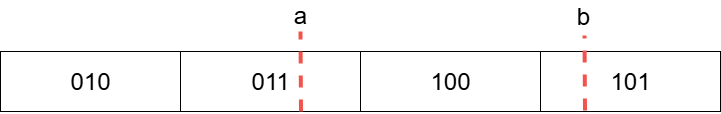
\includegraphics[width=12cm]{figuras/DiagramasTCC-Diagramas-Aritmetic-Rescaling-3Q}
    \fonte{Elaborada pelo autor}
\end{figure}

\begin{figure}[ht]
	\centering
	\caption{Subdivisão específica em \( \frac{1}{4} \)}
	\label{fig:DiagramasTCC-Diagramas-Aritmetic-Rescaling-Q}
	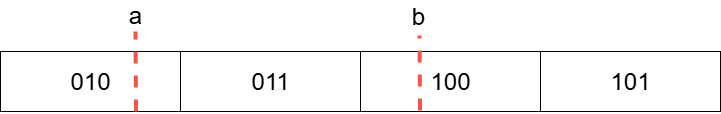
\includegraphics[width=12cm]{figuras/DiagramasTCC-Diagramas-Aritmetic-Rescaling-Q}
    \fonte{Elaborada pelo autor}
\end{figure}


Para fazer esta implementação da codificação aritmética com \textit{precisão finita}, define-se inicialmente a \textit{precisão} como o número de bits utilizados para representar os valores numéricos. Por exemplo, para uma precisão de \(p = 32\) bits, são definidos três valores auxiliares:
\[
\text{Todo} = 2^{p}, \quad \text{Metade} = \frac{\text{Todo}}{2}, \quad \text{quarto} = \frac{\text{Todo}}{4}.
\]

Seja o alfabeto de símbolos:
\[
\mathcal{X} = \{ 0, 1, \ldots, n \}, \quad \text{com um símbolo especial EoF} = 0.
\]
O vetor de probabilidades:
\[
p = (p_0, p_1, \ldots, p_n), \quad p_i = \frac{f_i}{\sum_{i=0}^{n} f_i},
\]
onde \(f_i\) representa a frequência observada para o símbolo \(i\).

Para inicialização, é necessário representar a variável \(R\) (\textit{range}) como um valor inteiro compatível com a precisão estabelecida.  
Seja a sequência de entrada \(x_1, x_2, \ldots, x_k \in \mathcal{X} \setminus \{ 0 \}\), com o símbolo \(x_{k+1} = 0\) representando o EoF.

Define-se:
\[
C_0 = 0, \quad C_j = r_0 + r_1 + \cdots + r_j, \quad \text{para } j = 1, \ldots, n,
\]
onde \(r_j\) representa o número acumulado de ocorrências (ou frequência acumulada) para os símbolos.

O vetor de deslocamento é dado por:
\[
d_j = c_j + r_j, \quad \text{para } j = 0, \ldots, n.
\]
Essas definições garantem que os intervalos de codificação e decodificação possam ser calculados corretamente utilizando aritmética inteira, preservando a precisão numérica durante todo o processo.


\newpage
\section{Biblioteca Komm}
A \textit{Komm} é uma biblioteca em \textit{Python} para sistemas de comunicação desenvolvida pelo professor Roberto Nobrega.  
Trata-se de um projeto \textit{open-source} para \textit{Python 3} que fornece ferramentas para análise e simulação de sistemas de comunicação analógicos e digitais.  

Este projeto foi inspirado em diversas outras bibliotecas para sistemas de comunicação, como \textit{MATLAB\textsuperscript{\textregistered} Communications System Toolbox\texttrademark}, \textit{GNU Radio}, \textit{CommPy} e \textit{SageMath}.  

Além disso, a biblioteca já disponibiliza diversas codificações implementadas, abrangendo diferentes técnicas de \textit{source coding} e \textit{lossless coding}, incluindo:  
\begin{itemize}
    \item {Shannon Code}
    \item {Fano Code}
    \item {Huffman Code}
    \item {Tunstal lCode}
    \item {LZ78}
    \item {LZW}
\end{itemize}
